\documentclass{beamer}
\usepackage{tikz}
\usepackage{float}
\usepackage{graphicx}
\usepackage[most]{tcolorbox}
\usepackage{comment}
\usepackage{bbm}
\usetikzlibrary{decorations.pathreplacing}
\tcbuselibrary{theorems}
\tcbset{enhanced,colframe=blue!20,colback={black!5!white},drop shadow}
\setbeamertemplate{section in toc}[sections numbered]
\setbeamertemplate{subsection in toc}[subsections numbered]
\usetheme[numbering=fraction]{metropolis}           % Use metropolis theme
\title{Bachelor Thesis Marginal-Sampling}
\date{\today}
\author{Michael Fedders}

\newcommand{\R}{\mathbb{R}}
\newcommand{\dx}{\, \mathrm{d}}
\begin{document}
	\maketitle
  	\begin{frame}[plain]
		\frametitle{Table of Contents}
		\tableofcontents
	\end{frame}
	
\section{Introduction}
	
	\begin{frame}{Model}
		We assume that we can describe a (biological) process through a function
		$x(t, \theta)$ with time $t$ and unknown model parameters $\theta$.
		Through (un)voluntary limitations the measured data is not $x$ but
		\[
			\overline{y} = c + h\bigl(x(t,\theta)\bigr) + \varepsilon
  		\]
		where
  		\begin{itemize}
  		\item $\overline{y}$ is the measured data
  		\item $c$ is an offset parameter
  		\item $h$ is the observation function
  		\item $\varepsilon$ is a noise - for now $\epsilon \sim \mathcal{N}(0, 
  		1/\lambda)$
  		\end{itemize}
	\end{frame}
	
	\begin{frame}{Standard approach}
		The standard approach is to use a data set $D$ to determine the model 
		parameters $\theta$ and the offset $c$ and noise parameter $\lambda$ with 			Bayes theorem:
		\[
			p(\theta,c,\lambda \mid D) = \frac{p(D \mid \theta,c,\lambda) \cdot
			p(\theta, c, \lambda)}{p(D)}.
		\]
		We can then use Markov chain Monte Carlo (MCMC) methods to proportionally 
		sample the posterior distribution with the product of \textbf{likelihood} 
		$p(D \mid \theta, c, \lambda)$ and \textbf{prior} $p(\theta, c, \lambda)$.
		We will call this way \textbf{FP-approach} from now on
	\end{frame}
	
	\begin{frame}{Hierarchical approach}
		For Maximum Likelihood methods it was shown that it can be faster to first 
		derive the model parameter $\theta$ and then in a second step the noise
		and transformation (e.g. offset, scaling) parameter [Loos, Krause, and
		 Hasenauer 2018] and [Schmiester et al. 2019].
		\begin{itemize}
			\item[$\implies$] We would like to apply the concept to posterior
			sampling. 
		\end{itemize}
	\end{frame}
	
	\begin{frame}{Hierarchical approach}
		For this \textbf{MP-approach} we use again Bayes theorem
		\[
			p(\theta \mid D) = \frac{p(D \mid \theta) \cdot
			p(\theta)}{p(D)}.
		\]
		If we can calculate the marginalized likelihood we can again use MCMC 
		methods to proportionally sample from the marginalized posterior 
		$p(\theta \mid D)$.
	\end{frame}
	
	\begin{frame}{Hierarchical approach}
		We calculate the required marginalized likelihood with
		\begin{align*}
			p(D \mid \theta) &= \iint p(D \mid \theta, c, \lambda) \cdot 
			p(\theta, c, \lambda) \dx c \dx \lambda.
		\end{align*}
	\end{frame}
	
	\begin{frame}[noframenumbering]{Hierarchical approach}
		We calculate the required marginalized likelihood with
		\begin{align*}
			p(D \mid \theta) &= \iint p(D \mid \theta, c, \lambda) \cdot 
			p(\theta, c, \lambda) \dx c \dx \lambda \\
			&= \iint p(D \mid \theta, c, \lambda) \cdot 
			p(c, \lambda) \dx c \dx \lambda \cdot p(\theta)
		\end{align*}
	\end{frame}
	

	
	\begin{frame}{MCMC}
		In our tests we used 2 different algorithms for the sampling, an adaptive 
		Metropolos sampler and a Parallel Tempering Sampler which is a multi chain 
		method. Every chain gets tempered with a temperature $\beta \in (0, 1]$ 
		i.e. instead of $p(D \mid \theta) \cdot p(\theta)$ we sample
		\[
			p(D \mid \theta)^\beta \cdot p(\theta).
		\]
		The first chain always has $\beta = 1$ such that it sample the correct 
		distribution. Then the different chains can exchange values - as the 
		chains with small $\beta$ sample a more uniform distribution we expect 
		more jumps which then lead to better mixing in the first chain.
	\end{frame}
	
	
	
\section{Gaussian noise}
  	
  	\begin{frame}{Normal-Gamma prior}
  		The normal-gamma prior depends on 4 shape parameters, $\mu \in \R, \kappa,
  		\alpha, \beta \in \R_+$ and has the following structure:
  		\begin{align*}
  			p(c, \lambda) &= f(c, \lambda \mid \mu, \kappa, \alpha, \beta) \\
  			&= \mathcal{N}(c \mid \mu, \hat{\lambda} = \kappa \lambda) \cdot 
  			\Gamma(\lambda \mid \alpha, \beta).
  		\end{align*}
  		For the prior $p(\theta)$ we will always consider a uniform distribution
  		for a reasonable large interval.
  		
  	\end{frame}
  	
  	\begin{frame}{Likelihood}
  		We recall that the measurements are defined as $\overline{y} = c + h +
  		\epsilon$. We assume independent noise for different points in time $t_1, 
  		\ldots, t_N, \ N \in \mathbb{N}$. Therefore the likelihood is
  		\begin{align*}
  			 p(D \mid \theta, c, \lambda) = \biggl(\frac{\lambda}{2\pi}\biggr) 
  			 ^{N/2} \cdot \exp\left( - \frac{\lambda}{2} \sum_{k = 1}^N 
  			 (\overline{y}_k - (c + h_k))^2 \right)
  		\end{align*}
  	\end{frame}
  	
	\begin{frame}{Marginal Likelihood}
  		The integral which we have to solve is defined as
  		\begin{align*}
    		p(D \mid \theta) &= \int_{\R \times \R_+} p(D \mid \theta,c,\lambda) 				p(c, \lambda) \, d(c, \lambda)
		\end{align*}
  	\end{frame}  	
  	
  	\begin{frame}[noframenumbering]{Marginal Likelihood}
  		The integral which we have to solve is defined as
  		\begin{align*}
    		p(D \mid \theta) =& \int_{\R \times \R_+} p(D \mid \theta,c,\lambda) 				p(c, \lambda) \, d(c, \lambda) \\
    		=& \int_{\R_+} \int_\R \biggl(\frac{\lambda}{2\pi}\biggr)^{N/2} \exp				\left( - \frac{\lambda}{2} \sum_{k = 1}^N (\overline{y}_k - (c +
    		h_k))^2 \right) \\
    		&\cdot \frac{\beta^\alpha \sqrt{\kappa}}{\Gamma(\alpha)\sqrt{2\pi}} 				\lambda^{\alpha-1/2} \exp\left(- \frac{\lambda}{2} \bigl(\kappa (c - 
    		\mu)^2 + 2\beta\bigr) \right) \, dc \, d\lambda
		\end{align*}
  	\end{frame}
  	
  	
\begin{comment}
  	\begin{frame}{Marginal Likelihood}
  		With an exponential integration formula
  		\[
  			\int_\R \exp(-a \cdot c^2 + b \cdot c - d) \, dc = \sqrt{\frac{\pi}					{a}} \cdot \exp \biggl( \frac{b^2}{4a} - d \biggr)
  		\]
  	\end{frame}
  	
  	\begin{frame}{Marginal Likelihood}
  		With an exponential integration formula
  		\[
  			\int_\R \exp(-a \cdot c^2 + b \cdot c - d) \, dc = \sqrt{\frac{\pi}					{a}} \cdot \exp \biggl( \frac{b^2}{4a} - d \biggr)
  		\]
  		and the substitution of $\varphi (\lambda) = C \cdot \lambda$ for
  		\begin{align*}
  			C \equiv& \ \frac{1}{2}\Biggl( \Biggl( \sum_{k = 1}^N (\overline{y_k}
  			 - h_k)^2 \Biggr) + \kappa \mu^2 + 2\beta \Biggr) \\
  			 &-  \frac{1}{2(N + \kappa)} \Biggl(\Biggl(\sum_{k = 1}^N
  			 \overline{y_k} - h_k\Biggr)+ \kappa \mu \Biggr)^2.
  		\end{align*}
  	\end{frame}  	
\end{comment}


  	\begin{frame}{Marginal Likelihood}
  		We recieve the following form:
  		\[
  			p(D \mid \theta) = \frac{(\beta / C)^\alpha}{\Gamma(\alpha) 
  			(2\pi C)^{\frac{N}{2}}} \cdot \sqrt{\frac{\kappa}{N + \kappa}}
  			\cdot \Gamma \biggl(\frac{N}{2} + \alpha \biggr)
  		\]
  		with
  		\begin{align*}
  			C \equiv& \ \frac{1}{2}\Biggl( \Biggl( \sum_{k = 1}^N (\overline{y_k}
  			 - h_k)^2 \Biggr) + \kappa \mu^2 + 2\beta \Biggr) \\
  			 &-  \frac{1}{2(N + \kappa)} \Biggl(\Biggl(\sum_{k = 1}^N
  			 \overline{y_k} - h_k\Biggr)+ \kappa \mu \Biggr)^2.
  		\end{align*}
   	\end{frame}
   	
   	\begin{frame}{Distribution of $c$ and $\lambda$}
   		To sample $c$ and $\lambda$ in a second step we need to derive their 
   		distribution from the integrand of the marginalized likelihood. We have
   		\[
   			\lambda \propto \operatorname{Gamma}(\alpha' = \alpha + N/2, \beta' 
   			= C)
   		\]
		and
		\[
			c \propto \mathcal{N} \left(\mu' = \frac{\left(\sum_{k = 1}^N
			\overline{y_k}-h_k \right) + \kappa \mu }{N + \kappa}, \hat{\lambda}
			= \lambda (N + \kappa) \right)
		\]
   	\end{frame}
   	
   	
\begin{comment}
\subsection{Conversion Reaction model}	
	
	\begin{frame}{Conversion Reaction model}
		For $k_1, k_2 \in \R$ we consider the following ordinary differential
		equation (ODE):
		\[
			\frac{d X_1(t)}{dt} = k_2 X_2 - k_1 X_1 \quad \quad 
			\frac{d X_2(t)}{dt} = k_2 X_1 - k_1 X_2.
		\]
		We want to observe $X_2$.
	\end{frame}
	
	\begin{frame}{Conversion Reaction model}
		For both approaches we sampled 50 independent runs with 10.000 steps each 
		with the Adaptive Metropolis sampler from pyPESTO. As underlying data we 
		used a toy data set of where we added an offset $c$ of 1.
	\end{frame}
	
	\begin{frame}{FP-approach}
		\begin{figure}
			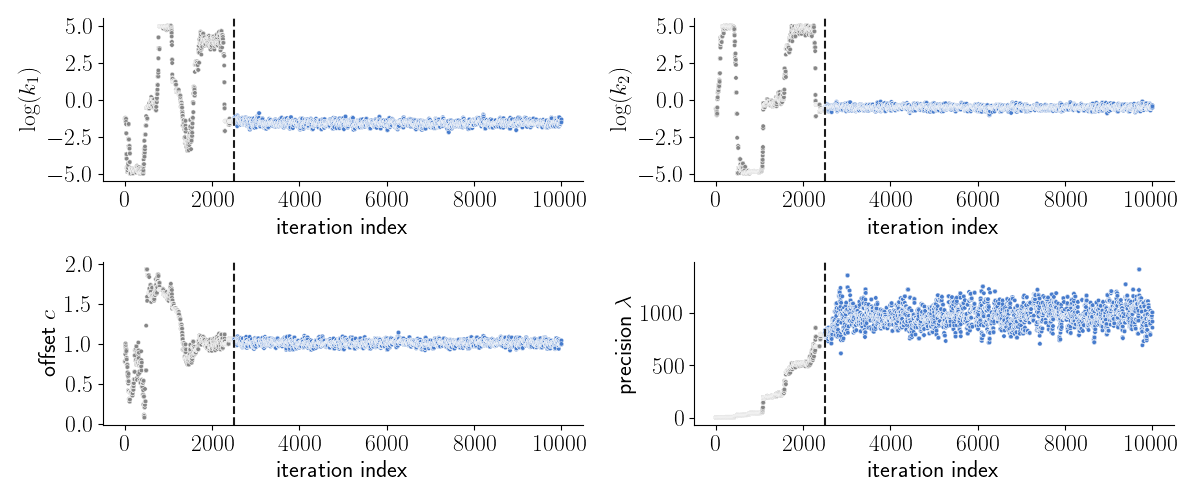
\includegraphics[width=1\columnwidth]
			{plots/CR_FP/parameters_CR_FP_30.png}
			\caption{One run with the FP-approach.}
		\end{figure}
	\end{frame}
	
	\begin{frame}{FP-approach}
		\begin{figure}
			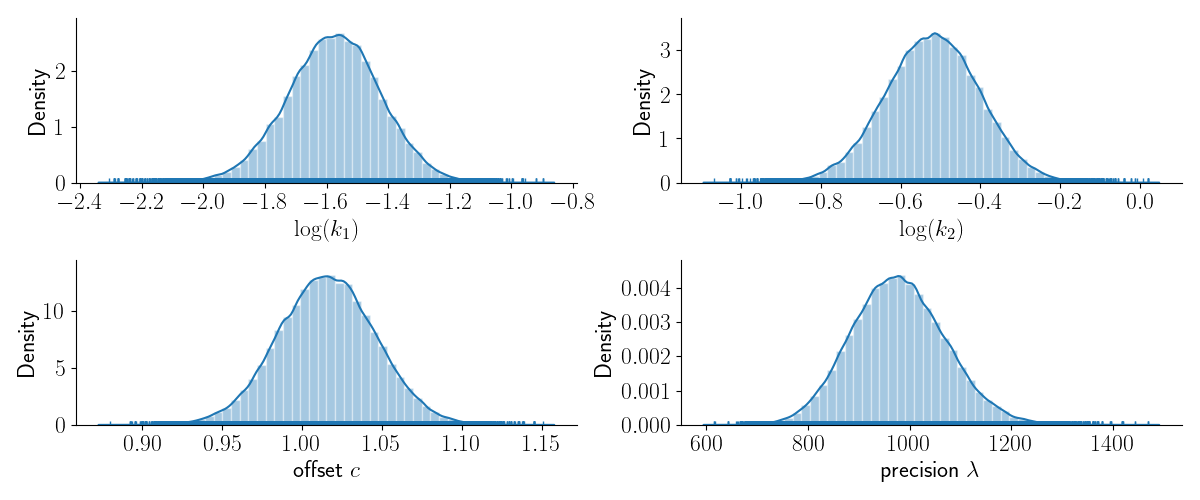
\includegraphics[width=1\columnwidth]
			{plots/CR_FP/merged_1d_marginals_CR_FP.png}
			\caption{Marginal densities from 50 independent runs with 
			FP-approach.}
		\end{figure}
	\end{frame}
	
	\begin{frame}{FP-approach}
		\begin{figure}
			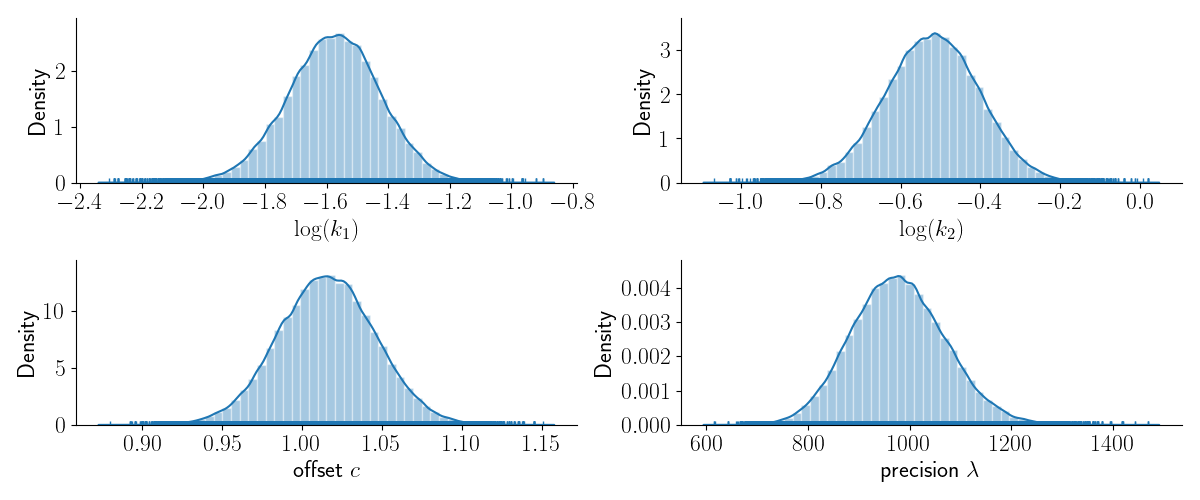
\includegraphics[width=1\columnwidth]
			{plots/CR_FP/merged_1d_marginals_CR_FP.png}
			\caption{Marginal densities from 50 independent runs with 
			FP-approach.}
		\end{figure}
		As a median we receive $\log(k_1) = -1.5765, \ \log(k_2) = -0.5180$
	\end{frame}
	
	\begin{frame}{FP-approach}
		\begin{figure}
			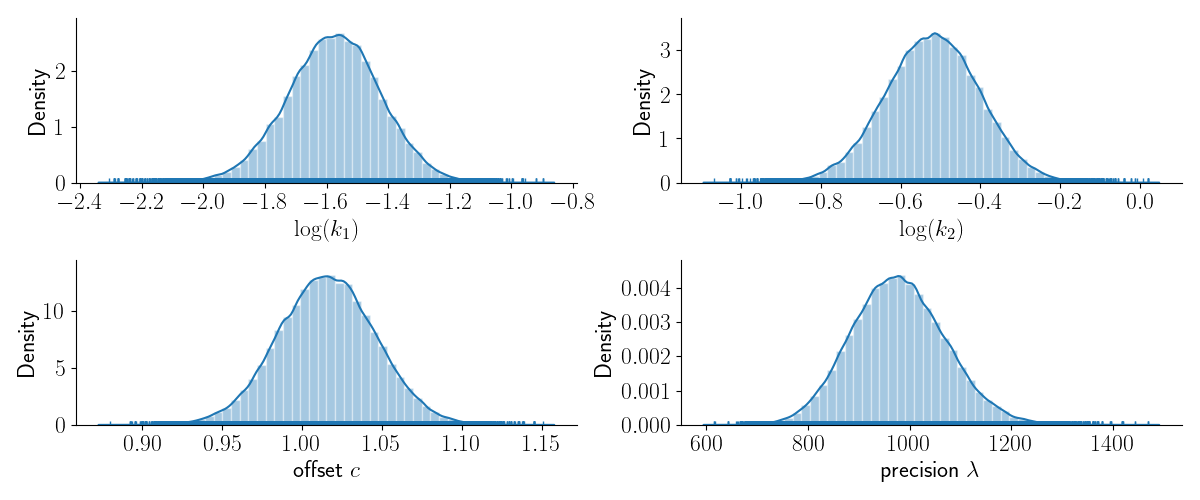
\includegraphics[width=1\columnwidth]
			{plots/CR_FP/merged_1d_marginals_CR_FP.png}
			\caption{Marginal densities from 50 independent runs with 
			FP-approach.}
		\end{figure}
		In linear scale $k_1 = 0.2067 , k_2 = 0.5957, c = 1.0148, \lambda = 975.44$
	\end{frame}
	
	\begin{frame}{FP-approach}
		\begin{figure}
			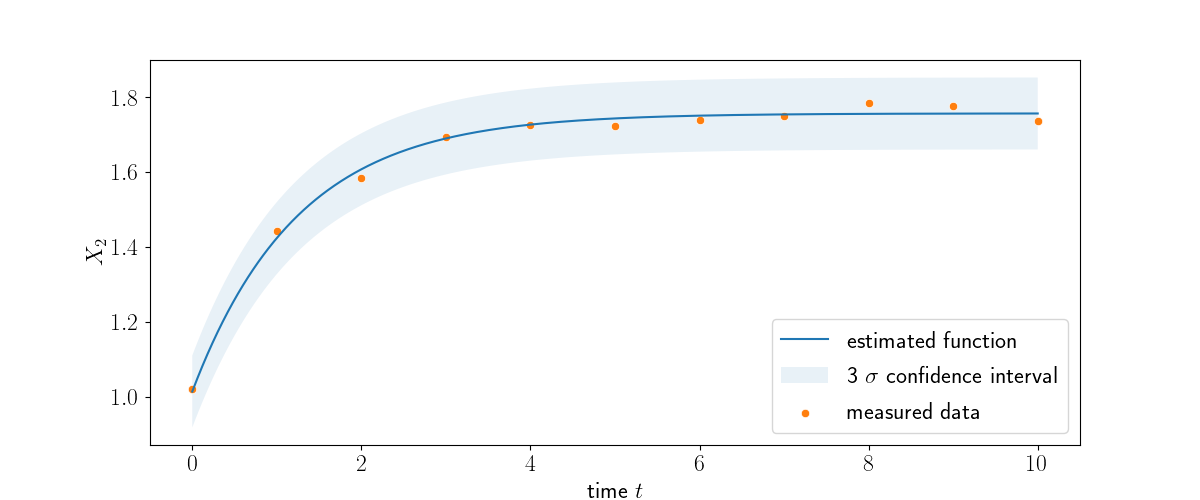
\includegraphics[width=1\columnwidth]
			{plots/combination/CR/comparison_data_estimate.png}
			\caption{Comparison of the estimated $X_2$ values with
			 the measured data, $\sigma = 1/\sqrt{\lambda} = 0,032$.}
		\end{figure}
	\end{frame}
	
	\begin{frame}{MP-approach}
		\begin{figure}
			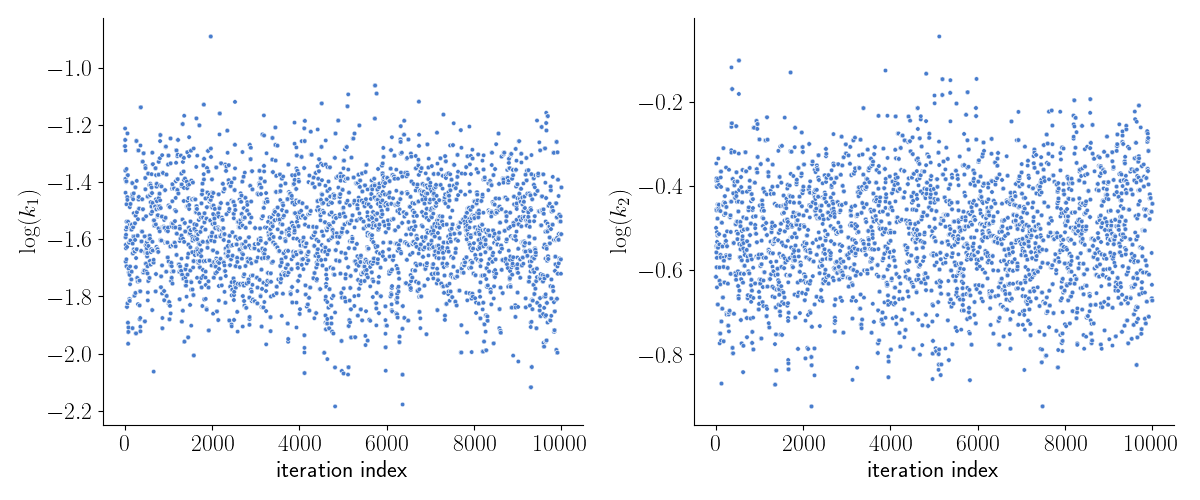
\includegraphics[width=1\columnwidth]
			{plots/CR_MP/parameters_CR_MP_30.png}
			\caption{One run for the MP-approach.}
		\end{figure}
	\end{frame}
	
	\begin{frame}{Comparison of both approaches}
		\begin{figure}
			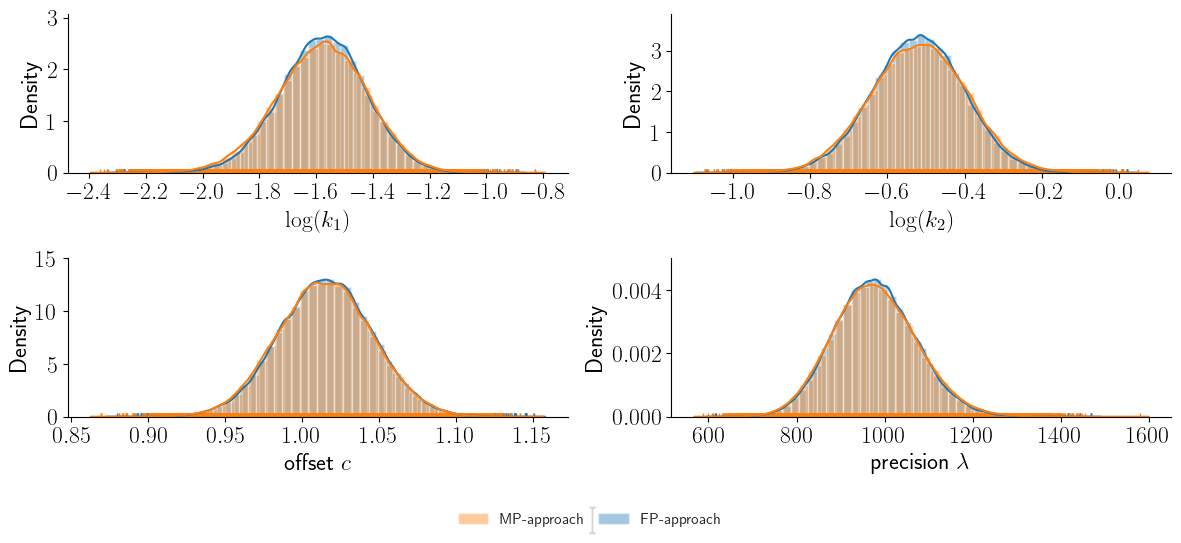
\includegraphics[width=1\columnwidth]
			{plots/combination/CR/overlap_plot_CR.png}
			\caption{Overlap for the marginal densities with both approaches.}
		\end{figure}
		$\implies$ We sampled the same densities.
	\end{frame}
	
	\begin{frame}{Comparison of FP-approach and MP-approach}
		\begin{figure}
			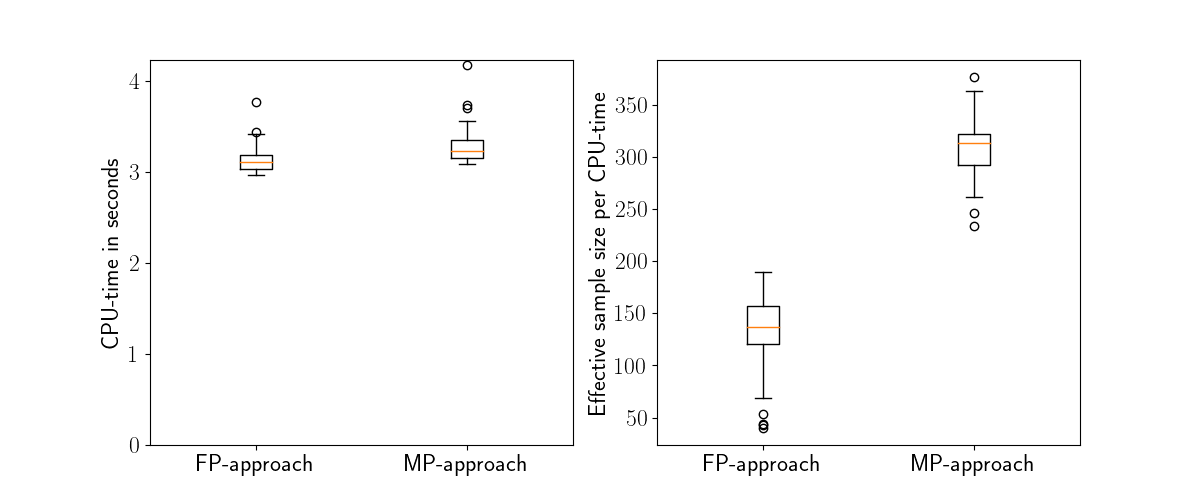
\includegraphics[width=1\columnwidth]
			{plots/combination/CR/Boxplot_only_theta_CR.png}
			\caption{Efficiency of both ways for sampling of $k_1$ and $k_2$.}
		\end{figure}
	\end{frame}
	
	\begin{frame}{Comparison of FP-approach and MP-approach}
		\begin{figure}
			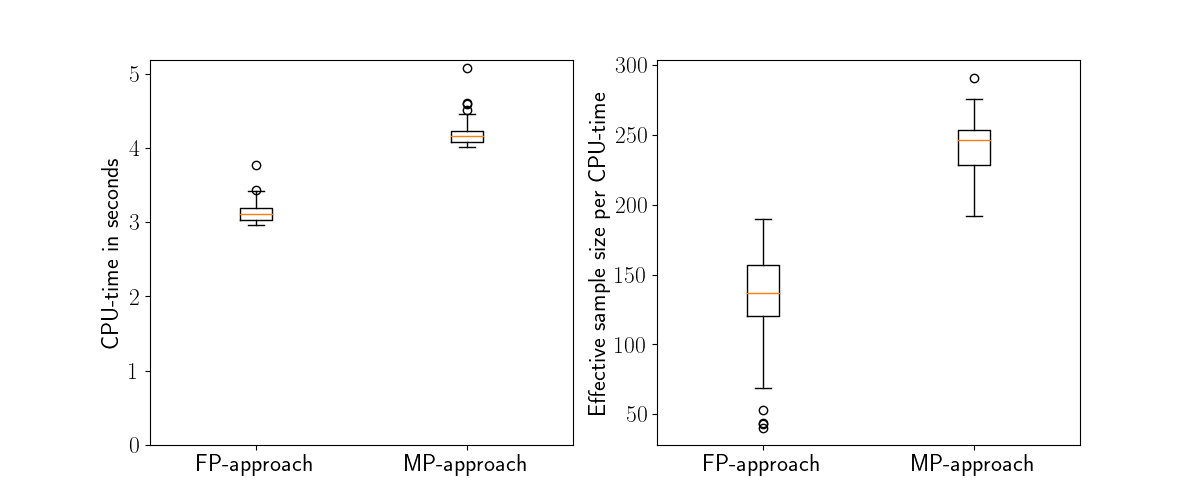
\includegraphics[width=1\columnwidth]
			{plots/combination/CR/Boxplot_all_CR.png}
			\caption{Efficiency of both ways when sampling all parameters}
		\end{figure}
	\end{frame}
\end{comment}


\subsection{mRNA-transfection model}
	
	\begin{frame}{mRNA-transfection model}
		For $\delta, \xi, k_{TL} \in \R$ we consider the mRNA-transfection model 
		which defines $x$ through
		\begin{align*}
    		\frac{d}{dt}X_1 = k_{TL} \cdot X_2 - \xi \cdot X_1 \quad \quad 
    		\text{and} \quad \frac{d}{dt}X_2 = -\delta \cdot X_2.
		\end{align*}
		In this model we will observe the value of $X_2$.
	\end{frame}
	
	\begin{frame}{Solutions}
		For an initial condition $X_1(t_1) = 0, \ X_2(t_1) = m_1$ we have the 
		analytical solution
		\[
			X_2(t, \theta = \{\delta, k_{TL} \cdot m_1, \xi, t_1\}) = 
			\frac{k_{TL} \cdot m_1}{\xi - \delta} \Bigl(e^{-\xi (t - t_1)} 
			- e^{-\delta(t - t_1)}\Bigr)
		\]
		Especially
		\[
			X_2(t, \delta = \delta_1, \xi = \xi_1) = X_2(t, \delta = \xi_1,
			 \xi = \delta_1)
		\]
	\end{frame}
	
	\begin{frame}{Sampling}
		As we are observing more variables and want to sample bimodal parameters 
		we increased the aomount of steps per run to 1.000.000 steps. As 
		underlying data we used experimental data and added an offset of 0,2. For 
		the sampling we used a Parallel Tempering algorithm from pyPESTO with 4 
		chains.
	\end{frame}
	
	\begin{frame}{FP-approach}
		\begin{figure}
			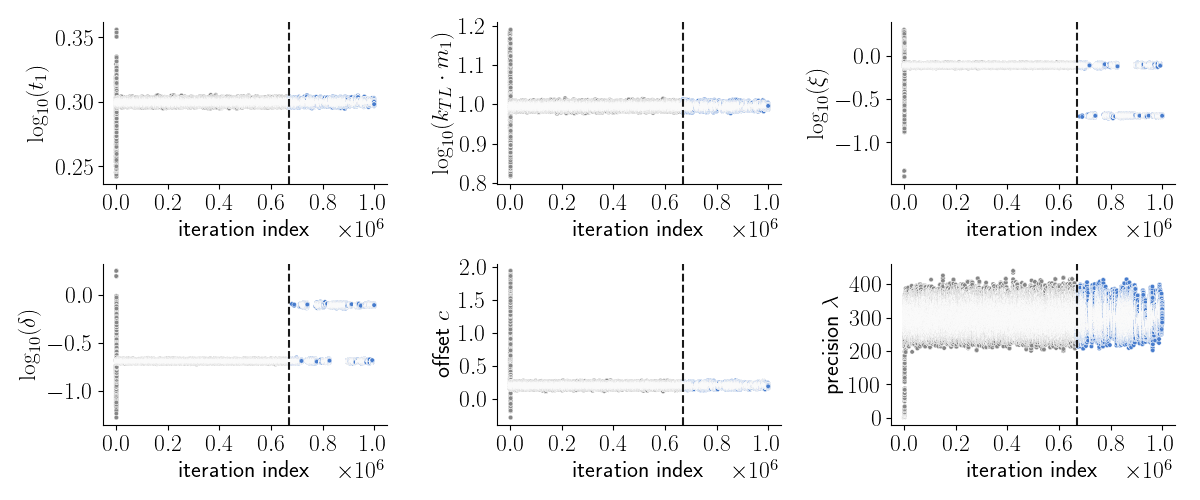
\includegraphics[width=1\columnwidth]
			{plots/mRNA_FP/parameters_mRNA_FP_2.png}
			\caption{A converging run for the FP-approach.}
		\end{figure}
	\end{frame}
	
	\begin{frame}{FP-approach}
		\begin{figure}
			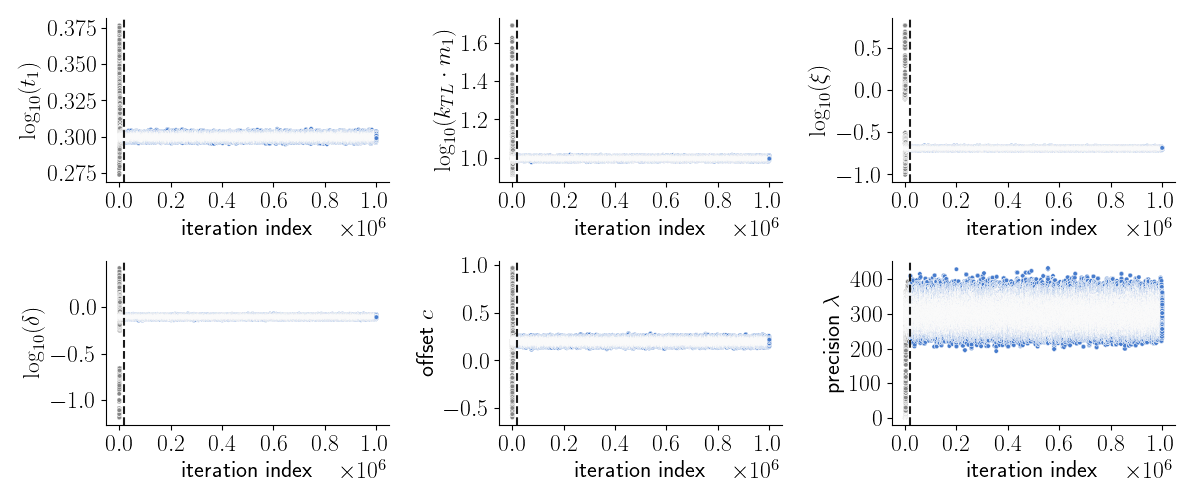
\includegraphics[width=1\columnwidth]
			{plots/mRNA_FP/parameters_mRNA_FP_7.png}
			\caption{A run which only samples in one mode.}
		\end{figure}
	\end{frame}
	
	\begin{frame}{FP-approach}
		\begin{figure}
			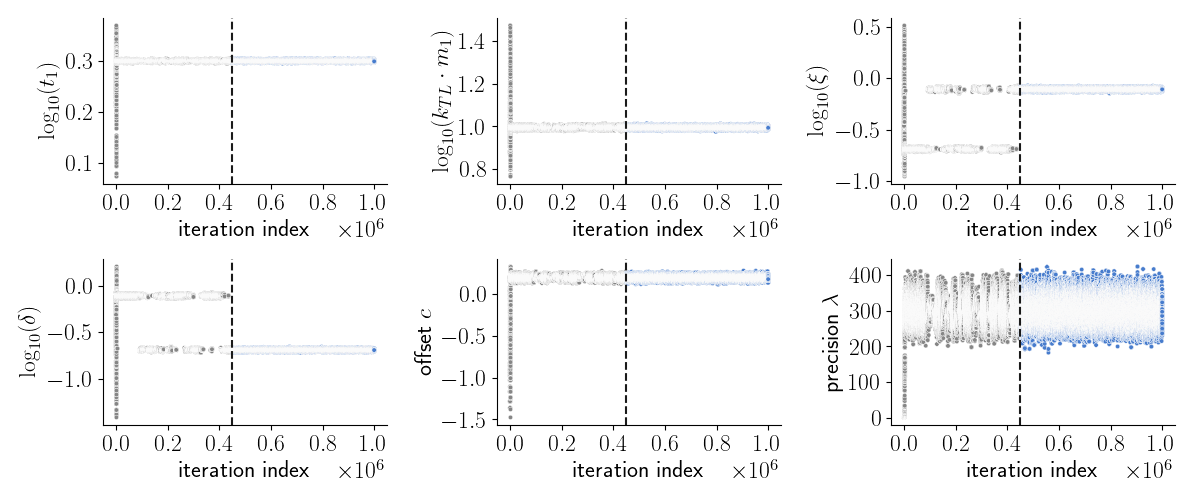
\includegraphics[width=1\columnwidth]
			{plots/mRNA_FP/parameter/parameters_mRNA_FP_28.png}
			\caption{A run which stops to sample in both modes.}
		\end{figure}
	\end{frame}
	
	\begin{frame}{FP-approach}
		\begin{figure}
			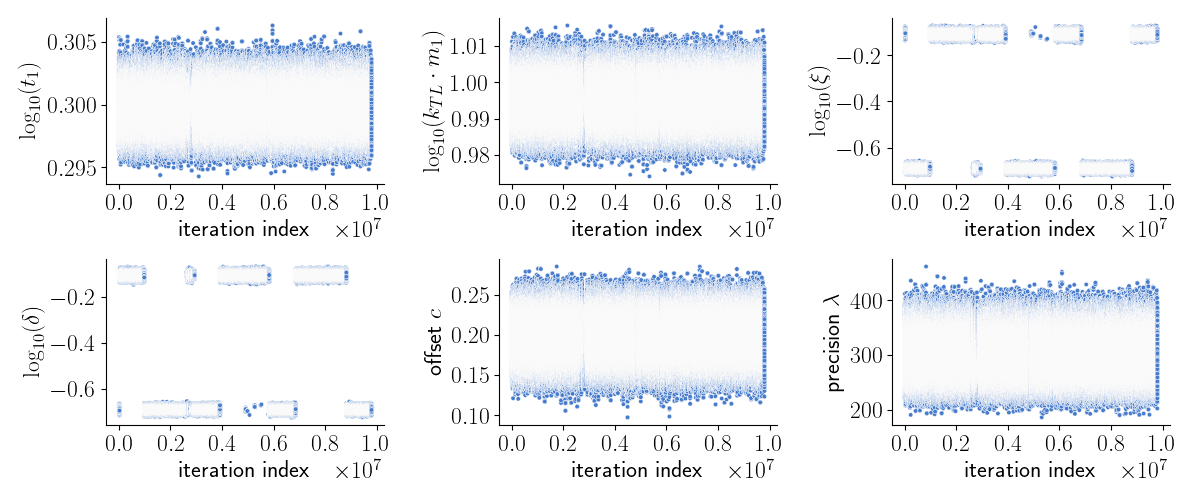
\includegraphics[width=1\columnwidth]
			{plots/mRNA_FP/merged_parameters_mRNA_FP.png}
			\caption{10 independent runs merged together.}
		\end{figure}
	\end{frame}
	
	\begin{frame}{FP-approach}
		\begin{figure}
			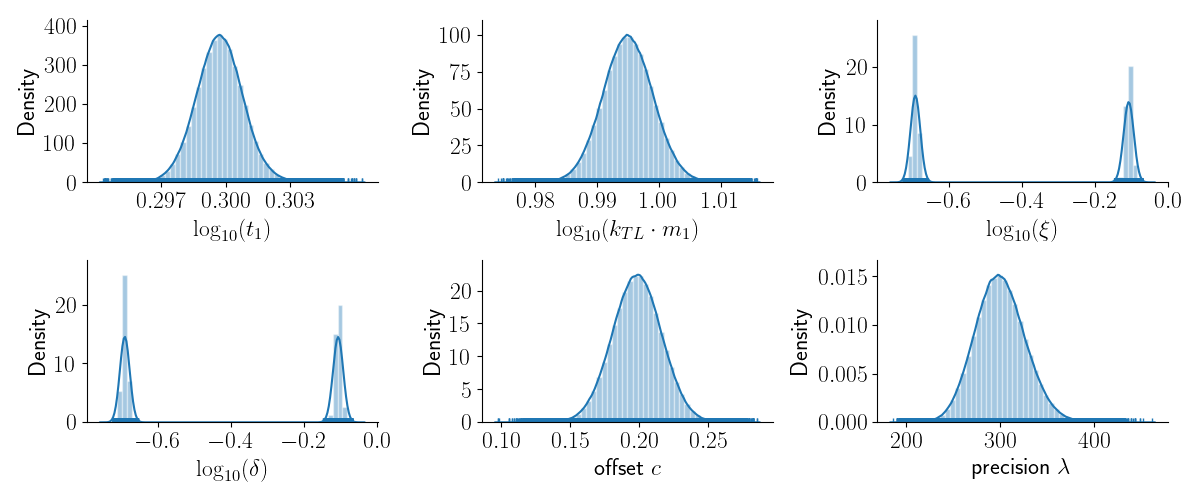
\includegraphics[width=1\columnwidth]
			{plots/mRNA_FP/merged_1d_marginals_mRNA_FP.png}
			\caption{The marginal densities for the 10 runs.}
		\end{figure}
		We can use the median for the parameters with one mode and take the 
		highest value separately for each mode for $\xi$ and $\delta$.
	\end{frame}
	
	\begin{frame}{FP-approach}
		We receive
		\begin{align*}
    		\log_{10}(t_1) &= 0.2997 &c = 0.9948 \\
    		\log_{10}(k_{TL} \cdot m_1) &= 0.1986 &\lambda = 299.80
		\end{align*}
		and two combiantions for $\xi$ and $\delta$:
		\begin{align*}
    		\log_{10}(\xi) = -0.1076 \ \text{and} \ \log_{10}(\delta) = -0.6909
		\end{align*}
		or
		\begin{align*}
    		\log_{10}(\xi) = -0.6909 \ \text{and} \ \log_{10}(\delta) = -0.1077.
		\end{align*}
	\end{frame}

	\begin{frame}{FP-approach}
		\begin{figure}
			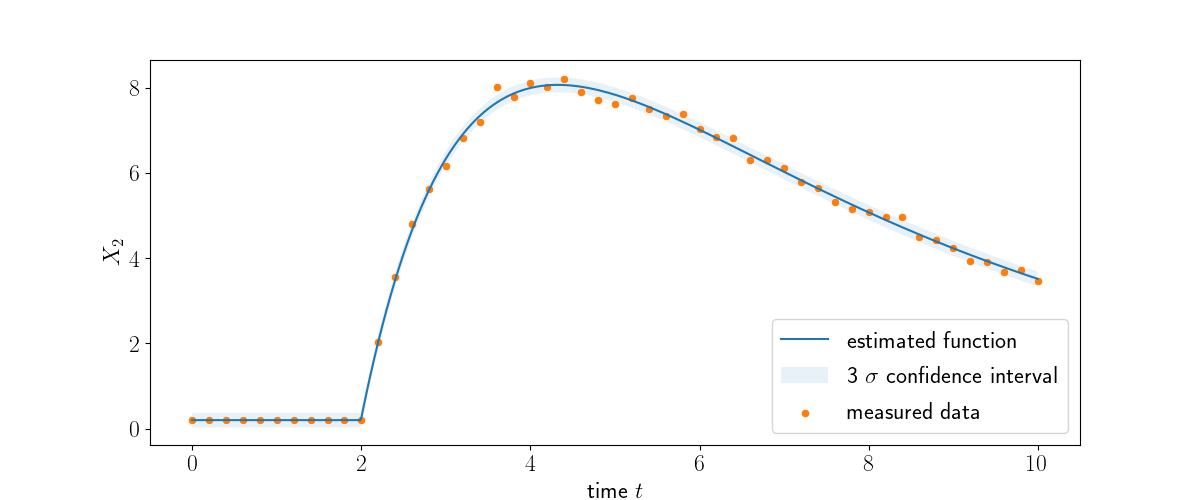
\includegraphics[width=1\columnwidth]
			{plots/combination/mRNA/comparison_data_estimate.png}
			\caption{Estimated value for $X_2$ and the easured data.}
		\end{figure}
	\end{frame}
	
	\begin{frame}{MP-approach}
		\begin{figure}
			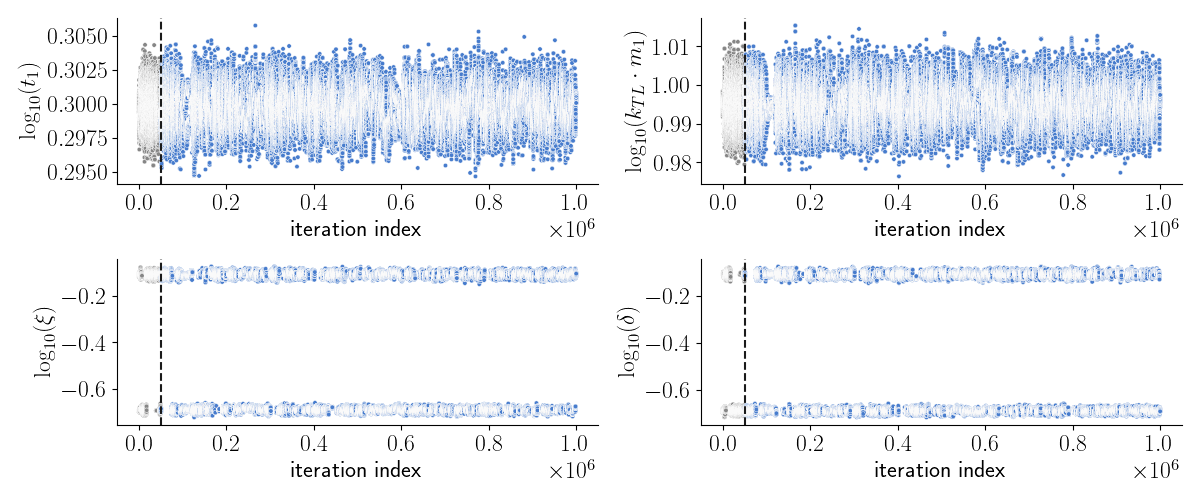
\includegraphics[width=1\columnwidth]
			{plots/mRNA_MP/parameters_mRNA_MP_5.png}
			\caption{One run with the MP-approach.}
		\end{figure}
	\end{frame}
	
	\begin{frame}{Comparison of both approaches}
		\begin{figure}
			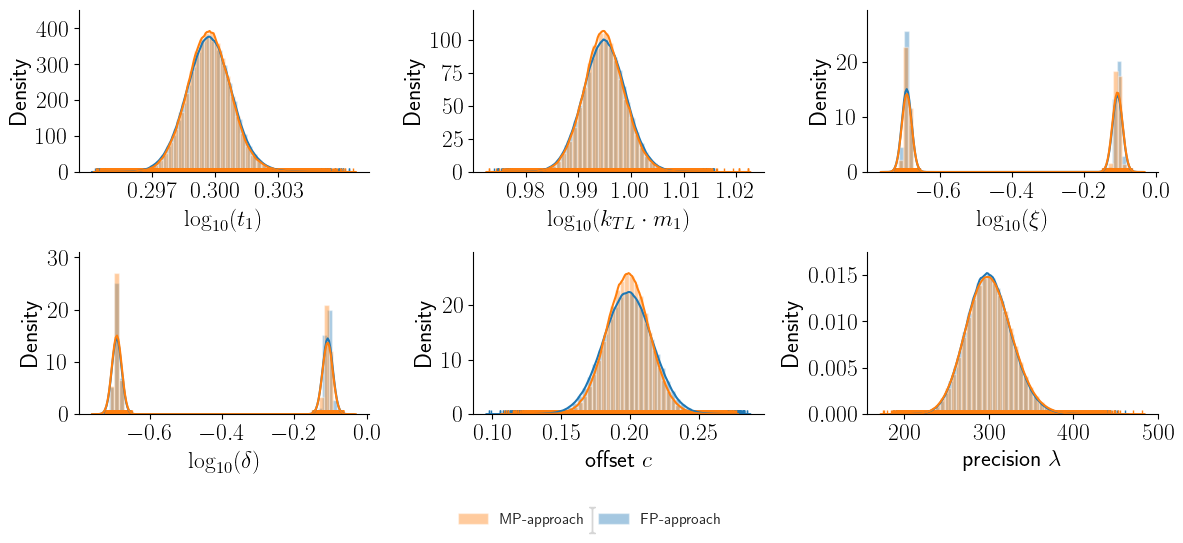
\includegraphics[width=1\columnwidth]
			{plots/combination/mRNA/overlap_plot_mRNA}
			\caption{Marginal densities for 10 independent runs each for both
			 approaches.}
		\end{figure}
	\end{frame}
	
	\begin{frame}{Comparison of both approaches}
		\begin{figure}
			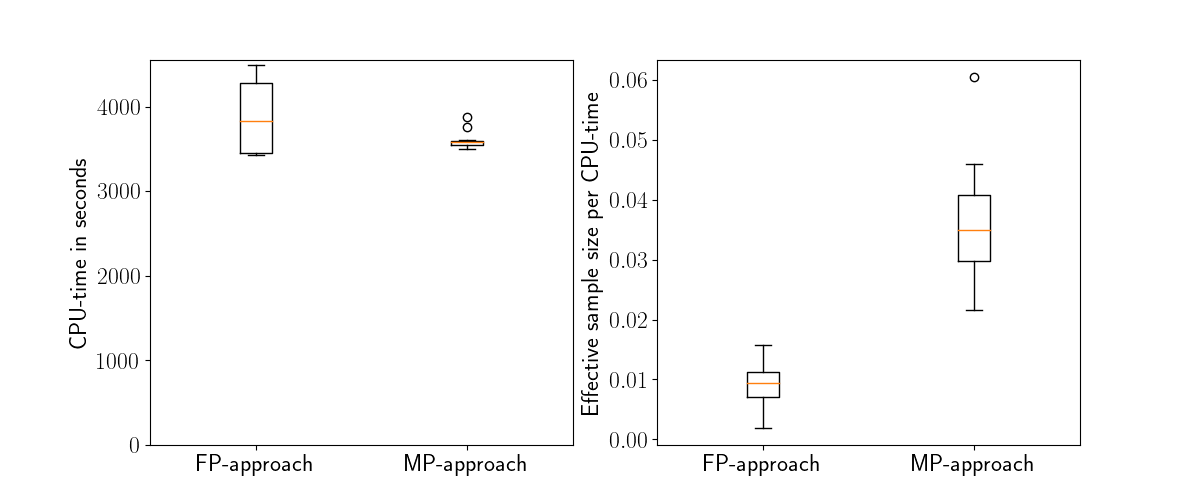
\includegraphics[width=1\columnwidth]
			{plots/combination/mRNA/Boxplot_only_theta_mRNA.png}
			\caption{Performance only for $\theta$ parameter and
			 \textbf{converged} runs.}
		\end{figure}
	\end{frame}
	
	\begin{frame}{Comparison of both approaches}
		\begin{figure}
			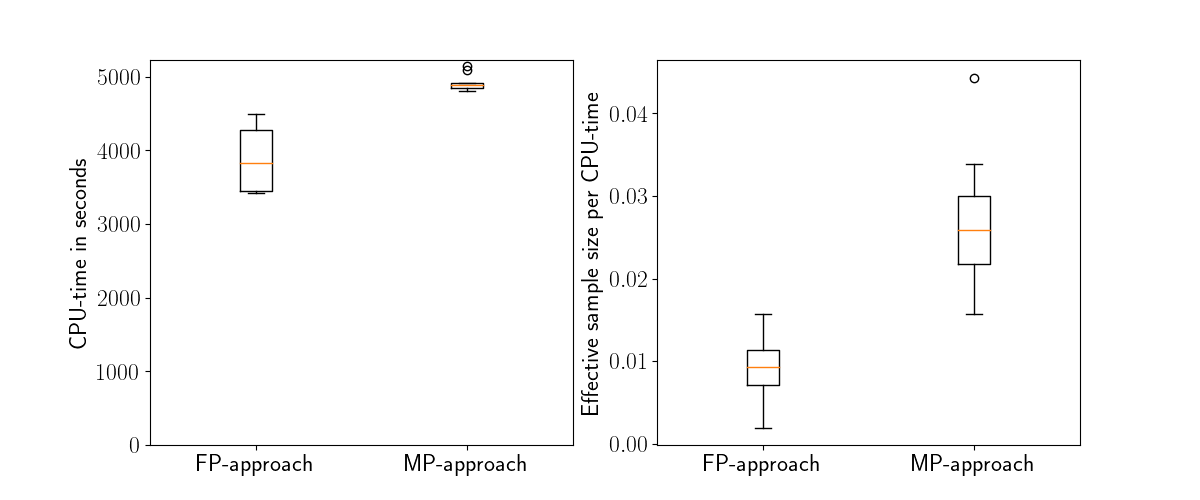
\includegraphics[width=1\columnwidth]
			{plots/combination/mRNA/Boxplot_all_mRNA.png}
			\caption{Performance for all parameters with \textbf{converged} runs.}
		\end{figure}
	\end{frame}

\section{Laplacian noise}

	\begin{frame}{Likelihood}
		Now we make the assumption that 
		\[
			\epsilon_k \sim Laplace(0, \sigma), \ \sigma \in (0, \infty)
		\]
		i.e. it has a Laplace distribution. The new likelihood has the following 
		form:
		\begin{align*}
    		p(D \mid \theta, c, \sigma) &= \prod_{k = 1}^N \operatorname{Laplace}
    		\ (\overline{y}_k	\mid c + h_k, \sigma) \\
    		&= \prod_{k = 1}^N \frac{1}{2\sigma} \cdot \exp \left\{- 							\frac{\lvert \overline{y}_k - c- h_k \lvert}{\sigma} \right\}
		\end{align*}
	\end{frame}
	
	\begin{frame}{Marginalised likelihood}
		The integral we receive is

		\begin{align*}
    		&\iint p(D \mid \theta, c, \sigma) p(c) p(\sigma) \dx c \dx \sigma \\
    		=& \int_0^{\infty} \int_{-\infty}^{\infty} \left( \prod_{k = 1}^N 					\frac{1}{2\sigma} \cdot \exp \left\{- \frac{|c - (\overline{y}_k 
    		-h_k)|} {\sigma} \right\} \right) p(c) p(\sigma) \dx c \dx \sigma
		\end{align*}
	\end{frame}
	
	\begin{frame}{Marginalised likelihood}
		For $b_0 = -\infty, \ b_i = \overline{y}_i - h_i \ (i = 1, \ldots, N), \
		b_{N+1} = \infty$ we can split up the integral in the following parts:
		\begin{align*}
    		\int_0^{\infty} \frac{p(\sigma)}{2\sigma} \sum_{i = 0}^N 
    		\int_{b_i}^{b_{i+1}} \exp \left\{- \frac{\sum_{k = 1}^N \lvert c -
    		(\overline{y}_k - h_k) \lvert} {\sigma} \right\} p(c)\dx c \dx \sigma.
		\end{align*}
	\end{frame}
	
	\begin{frame}{Marginalised likelihood}
		We finally receive
		\begin{align*}
    		&\int_0^\infty \frac{p(\sigma)}{2\sigma} \Biggl( \sum_{i = 0}^N 
    		\exp \left\{\frac{\bigl( \sum_{k = 1}^i \overline{y}_k - h_k \bigr) - 
    		\bigl( \sum_{k = i + 1}^N \overline{y}_k - h_k \bigr)}{\sigma}
    		\right\} \\
    		&\cdot \int_{b_i}^{b_{i + 1}} e^{c \cdot (N - 2i)} p(c) \dx c \Biggr) 
    		\dx \sigma
		\end{align*}
	\end{frame}
	
	\begin{frame}{Marginalised likelihood}
		With
		\[
			l_i \equiv \left( \sum_{k = 1}^i \overline{y}_k - h_k \right ) - 
			\left( \sum_{k = i + 1}^N \overline{y}_k - h_k \right ) \quad 
			\text{for} \; i = 0, \ldots, N.
		\]
		we can write the integral as
		\[
			\sum_{i = 0}^N \int_0^\infty \frac{p(\sigma)}{2\sigma} \exp \left \{
			\frac{l_i}{\sigma} \right \} \int_{b_i}^{b_{i + 1}} e^{c \cdot 
			(N - 2i)} p(c) \dx c
		\]
	\end{frame}
	
	\begin{frame}{Exponential $c$ prior}
		We were not aware of any standard choice for the priors so we tried out 
		different possibilities. We will start with an exponential distribution, 
		i.e.
		\[		
			p(c) = \lambda e^{-\lambda\cdot c} \; \text{with} \; \lambda > 0.
		\]
	\end{frame}
	
	\begin{frame}[noframenumbering]{Exponential $c$ prior}
		We were not aware of any standard choice for the priors so we tried out 
		different possibilities. We will start with an exponential distribution, 
		i.e.
		\[		
			p(c) = \lambda e^{-\lambda\cdot c} \; \text{with} \; \lambda > 0.
		\]
		The integral becomes
		\[
			\int_0^\infty \frac{\lambda \cdot p(\sigma)}{2\sigma}  \sum_{i = 0}^N 
			e^{l_i/\sigma} \int_{b_i}^{b_{i + 1}} \mathbbm{1}_{[0, \infty)}(c) 
			\cdot e^{-c(2i -N + \lambda)} \dx c \dx \sigma.
		\]
	\end{frame}
	
	\begin{frame}{Exponential $c$ prior}
	Let $r = \min\{i = 0, \ldots, N \mid b_i \geq 0\}$. We also introduce the 
	notation	
		\begin{align*}
			b_{0, \ldots, r-1} &\equiv 0 \\
    		b_r &\equiv \frac{\lambda}{2(N -2r - \lambda)} \cdot \Bigl( 
    		e^{b_{r + 1} (N -2r - \lambda)} - 1 \Bigr) \\
    		b_{i = r + 1, \ldots, N - 1} &\equiv e^{l_i/\sigma} \frac{\lambda}{2(N 
    		- 2i - \lambda)}\Bigl(e^{b_{i + 1} (N -2(i+1) - \lambda)} - e^{b_i 
    		(N -2i - \lambda)} \Bigr) \\
    		b_N &\equiv e^{l_N/\sigma} \frac{\lambda}{2(N + \lambda)} e^{-b_N 
    		(N + \lambda)}.
		\end{align*}
	\end{frame}
	
	\begin{frame}{$c$ prior}
		We finally have
		\[
			p(D \mid \theta) = \sum_{i = 0}^N b_i \int_0^\infty \frac{p(\sigma)}
			{\sigma} \exp \biggl\{\frac{l_i}{\sigma} \biggr\} \dx \sigma.
		\]
		In general also for a Gaussian or Laplacian $c$ prior we arrive at such a form 
		just with different constants (and possibly different support).
	\end{frame}
	
	\begin{frame}{Amoroso $\sigma$ prior}
		For $a, b \neq 0, c \in \R$ and $d \in \R_+$ we have
		\begin{align*}
    		\operatorname{Amoroso}(\sigma \mid a, b, c, d) = \frac{1}{\Gamma(d)} 				\bigg \lvert \frac{c}{b} \bigg \lvert \left( \frac{\sigma - a}{b} 					\right)^{d\cdot c - 1} \exp \biggl\{- \left(\frac{\sigma - a}{b} 					\right)^c \biggr\}
		\end{align*}
		with $\operatorname{supp}(\sigma) = [a, \infty)$ if $b > 0$ and $					\operatorname{supp}(\sigma) = (-\infty, a]$ if $b < 0$.
		\begin{itemize}
			\item[$\implies$]We will use $d = 1, c = -2, b = 1, a = 0$.
		\end{itemize}
	\end{frame}
	
	\begin{frame}{Amoroso $\sigma$ prior}
		We need $a = 0$ for the correct support and $c < -1$ so that our integral 
		converges, the other values are chose to simplify the calculation and can 
		be generalized. The prior has the form
		\[
			p(\sigma) = 2 \cdot \sigma^{-3} \exp\biggl\{ -\frac{1}{\sigma^2}
			\biggr\}
		\]
		and therefore the integral has the form
		\[
			\sum_{i = 0}^N  \int_0^\infty \frac{2 b_i} {\sigma^4} \exp 
			\biggl\{\frac{l_i}{\sigma} - \frac{1}{\sigma^2} \biggr\} \dx \sigma.
		\]
	\end{frame}
	
\section{Outlook}
	\begin{frame}{Outlook}
		There are several parts which can be extended.
	\end{frame}
	
	\begin{frame}[noframenumbering]{Outlook}
		There are several parts which can be extended.
		\begin{itemize}
			\item In the same setting we can test the efficiency for the Gaussian 
			noise in more complex models.
		\end{itemize}
	\end{frame}
	
	\begin{frame}[noframenumbering]{Outlook}
		There are several parts which can be extended.
		\begin{itemize}
			\item In the same setting we can test the efficiency for the Gaussian 
			noise in more complex models.
			\item For the Laplacian noise we can finish the derivation and start 
			the tests with models as well.
		\end{itemize}
	\end{frame}
	
	\begin{frame}[noframenumbering]{Outlook}
		There are several parts which can be extended.
		\begin{itemize}
			\item In the same setting we can test the efficiency for the Gaussian 
			noise in more complex models.
			\item For the Laplacian noise we can finish the derivation and start 
			the tests with models as well.
			\item Also we can extend the setting to also include scaling 
			parameters.
		\end{itemize}
	\end{frame}
	
	\begin{frame}{End}
		Thank you for your attention!
	\end{frame}
	
\end{document}





















